% Options for packages loaded elsewhere
\PassOptionsToPackage{unicode}{hyperref}
\PassOptionsToPackage{hyphens}{url}
%
\documentclass[
]{article}
\usepackage{amsmath,amssymb}
\usepackage{lmodern}
\usepackage{iftex}
\ifPDFTeX
  \usepackage[T1]{fontenc}
  \usepackage[utf8]{inputenc}
  \usepackage{textcomp} % provide euro and other symbols
\else % if luatex or xetex
  \usepackage{unicode-math}
  \defaultfontfeatures{Scale=MatchLowercase}
  \defaultfontfeatures[\rmfamily]{Ligatures=TeX,Scale=1}
\fi
% Use upquote if available, for straight quotes in verbatim environments
\IfFileExists{upquote.sty}{\usepackage{upquote}}{}
\IfFileExists{microtype.sty}{% use microtype if available
  \usepackage[]{microtype}
  \UseMicrotypeSet[protrusion]{basicmath} % disable protrusion for tt fonts
}{}
\makeatletter
\@ifundefined{KOMAClassName}{% if non-KOMA class
  \IfFileExists{parskip.sty}{%
    \usepackage{parskip}
  }{% else
    \setlength{\parindent}{0pt}
    \setlength{\parskip}{6pt plus 2pt minus 1pt}}
}{% if KOMA class
  \KOMAoptions{parskip=half}}
\makeatother
\usepackage{xcolor}
\usepackage[margin=1in]{geometry}
\usepackage{color}
\usepackage{fancyvrb}
\newcommand{\VerbBar}{|}
\newcommand{\VERB}{\Verb[commandchars=\\\{\}]}
\DefineVerbatimEnvironment{Highlighting}{Verbatim}{commandchars=\\\{\}}
% Add ',fontsize=\small' for more characters per line
\usepackage{framed}
\definecolor{shadecolor}{RGB}{248,248,248}
\newenvironment{Shaded}{\begin{snugshade}}{\end{snugshade}}
\newcommand{\AlertTok}[1]{\textcolor[rgb]{0.94,0.16,0.16}{#1}}
\newcommand{\AnnotationTok}[1]{\textcolor[rgb]{0.56,0.35,0.01}{\textbf{\textit{#1}}}}
\newcommand{\AttributeTok}[1]{\textcolor[rgb]{0.77,0.63,0.00}{#1}}
\newcommand{\BaseNTok}[1]{\textcolor[rgb]{0.00,0.00,0.81}{#1}}
\newcommand{\BuiltInTok}[1]{#1}
\newcommand{\CharTok}[1]{\textcolor[rgb]{0.31,0.60,0.02}{#1}}
\newcommand{\CommentTok}[1]{\textcolor[rgb]{0.56,0.35,0.01}{\textit{#1}}}
\newcommand{\CommentVarTok}[1]{\textcolor[rgb]{0.56,0.35,0.01}{\textbf{\textit{#1}}}}
\newcommand{\ConstantTok}[1]{\textcolor[rgb]{0.00,0.00,0.00}{#1}}
\newcommand{\ControlFlowTok}[1]{\textcolor[rgb]{0.13,0.29,0.53}{\textbf{#1}}}
\newcommand{\DataTypeTok}[1]{\textcolor[rgb]{0.13,0.29,0.53}{#1}}
\newcommand{\DecValTok}[1]{\textcolor[rgb]{0.00,0.00,0.81}{#1}}
\newcommand{\DocumentationTok}[1]{\textcolor[rgb]{0.56,0.35,0.01}{\textbf{\textit{#1}}}}
\newcommand{\ErrorTok}[1]{\textcolor[rgb]{0.64,0.00,0.00}{\textbf{#1}}}
\newcommand{\ExtensionTok}[1]{#1}
\newcommand{\FloatTok}[1]{\textcolor[rgb]{0.00,0.00,0.81}{#1}}
\newcommand{\FunctionTok}[1]{\textcolor[rgb]{0.00,0.00,0.00}{#1}}
\newcommand{\ImportTok}[1]{#1}
\newcommand{\InformationTok}[1]{\textcolor[rgb]{0.56,0.35,0.01}{\textbf{\textit{#1}}}}
\newcommand{\KeywordTok}[1]{\textcolor[rgb]{0.13,0.29,0.53}{\textbf{#1}}}
\newcommand{\NormalTok}[1]{#1}
\newcommand{\OperatorTok}[1]{\textcolor[rgb]{0.81,0.36,0.00}{\textbf{#1}}}
\newcommand{\OtherTok}[1]{\textcolor[rgb]{0.56,0.35,0.01}{#1}}
\newcommand{\PreprocessorTok}[1]{\textcolor[rgb]{0.56,0.35,0.01}{\textit{#1}}}
\newcommand{\RegionMarkerTok}[1]{#1}
\newcommand{\SpecialCharTok}[1]{\textcolor[rgb]{0.00,0.00,0.00}{#1}}
\newcommand{\SpecialStringTok}[1]{\textcolor[rgb]{0.31,0.60,0.02}{#1}}
\newcommand{\StringTok}[1]{\textcolor[rgb]{0.31,0.60,0.02}{#1}}
\newcommand{\VariableTok}[1]{\textcolor[rgb]{0.00,0.00,0.00}{#1}}
\newcommand{\VerbatimStringTok}[1]{\textcolor[rgb]{0.31,0.60,0.02}{#1}}
\newcommand{\WarningTok}[1]{\textcolor[rgb]{0.56,0.35,0.01}{\textbf{\textit{#1}}}}
\usepackage{graphicx}
\makeatletter
\def\maxwidth{\ifdim\Gin@nat@width>\linewidth\linewidth\else\Gin@nat@width\fi}
\def\maxheight{\ifdim\Gin@nat@height>\textheight\textheight\else\Gin@nat@height\fi}
\makeatother
% Scale images if necessary, so that they will not overflow the page
% margins by default, and it is still possible to overwrite the defaults
% using explicit options in \includegraphics[width, height, ...]{}
\setkeys{Gin}{width=\maxwidth,height=\maxheight,keepaspectratio}
% Set default figure placement to htbp
\makeatletter
\def\fps@figure{htbp}
\makeatother
\setlength{\emergencystretch}{3em} % prevent overfull lines
\providecommand{\tightlist}{%
  \setlength{\itemsep}{0pt}\setlength{\parskip}{0pt}}
\setcounter{secnumdepth}{-\maxdimen} % remove section numbering
\newlength{\cslhangindent}
\setlength{\cslhangindent}{1.5em}
\newlength{\csllabelwidth}
\setlength{\csllabelwidth}{3em}
\newlength{\cslentryspacingunit} % times entry-spacing
\setlength{\cslentryspacingunit}{\parskip}
\newenvironment{CSLReferences}[2] % #1 hanging-ident, #2 entry spacing
 {% don't indent paragraphs
  \setlength{\parindent}{0pt}
  % turn on hanging indent if param 1 is 1
  \ifodd #1
  \let\oldpar\par
  \def\par{\hangindent=\cslhangindent\oldpar}
  \fi
  % set entry spacing
  \setlength{\parskip}{#2\cslentryspacingunit}
 }%
 {}
\usepackage{calc}
\newcommand{\CSLBlock}[1]{#1\hfill\break}
\newcommand{\CSLLeftMargin}[1]{\parbox[t]{\csllabelwidth}{#1}}
\newcommand{\CSLRightInline}[1]{\parbox[t]{\linewidth - \csllabelwidth}{#1}\break}
\newcommand{\CSLIndent}[1]{\hspace{\cslhangindent}#1}
\usepackage{fancyhdr}
\pagestyle{fancy}
% center of header
\fancyhead[CO,CE]{Bioestadística en R -Módulo 1 : Análisis de la diversidad}
\rhead{
\includegraphics[width = .15\textwidth]{imagenes/ctbc.jpg}}
% center of footer
\fancyfoot[C]{\textbf{--~\thepage~--}}% page number on the left of even pages and right of odd pages
%\fancyfoot[LE,RO]{\thepage}
%\cfoot{
\includegraphics[width = 12\textwidth]{imagenes/logo2.png}}
\ifLuaTeX
  \usepackage{selnolig}  % disable illegal ligatures
\fi
\IfFileExists{bookmark.sty}{\usepackage{bookmark}}{\usepackage{hyperref}}
\IfFileExists{xurl.sty}{\usepackage{xurl}}{} % add URL line breaks if available
\urlstyle{same} % disable monospaced font for URLs
\hypersetup{
  pdftitle={Bioestadística en R - parte práctica clase 1, Módulo 1 : Análisis de la diversidad.},
  pdfauthor={Ph D. Stephanie Hereira Pacheco},
  hidelinks,
  pdfcreator={LaTeX via pandoc}}

\title{Bioestadística en R - parte práctica clase 1, Módulo 1 : Análisis
de la diversidad.}
\author{Ph D. Stephanie Hereira Pacheco}
\date{}

\begin{document}
\maketitle

{
\setcounter{tocdepth}{3}
\tableofcontents
}
\hypertarget{parte-1}{%
\section{Parte 1}\label{parte-1}}

El propósito de este cuadernillo es aplicar el cálculo u obtención de
algunos conocimientos teóricos impartidos en la clase 1 en el módulo I
del curso de Bioestadística en R. Hay varios paquetes y funciones en R
que nos permitirán explorar nuestros datos ecológicos. Inicialmente
veremos cómo calcular los índices de diversidad en el marco de los
números de Hill utilizando el paquete \texttt{hillR} , luego
exploraremos el paquete \texttt{betapart} que nos permitirá obtener la
partición de la diversidad beta. De igual forma trataremos revisaremos
un poco del paquete \texttt{vegan} que nos permite calcular otros
índices de diversidad y otras matrices de distancia de la diversidad
beta.

\hypertarget{hillr1}{%
\subsection[\texttt{hillR}]{\texorpdfstring{\texttt{hillR}\footnote{\url{https://github.com/daijiang/hillR}}}{hillR}}\label{hillr1}}

El paquete \texttt{hillR} contiene funciones para calcular la diversidad
taxonómica, funcional y filogenética en el marco de los números de Hill.
Los métodos están basados en la referencia (Chao, Chiu, and Jost 2014)
que ya hemos tratado en la parte teórica.

Para instalar este paquete usamos el comando:

\begin{Shaded}
\begin{Highlighting}[]
\FunctionTok{install.packages}\NormalTok{(}\StringTok{"hillR"}\NormalTok{)}
\CommentTok{\# o instala la versión en desarrollo del github}
\NormalTok{devtools}\SpecialCharTok{::}\FunctionTok{install\_github}\NormalTok{(}\StringTok{"daijiang/hillR"}\NormalTok{)}
\end{Highlighting}
\end{Shaded}

También instalaremos el paquete \texttt{FD} de dónde usaremos la data
ejemplo:

\begin{Shaded}
\begin{Highlighting}[]
\FunctionTok{install.packages}\NormalTok{(}\StringTok{"FD"}\NormalTok{)}
\end{Highlighting}
\end{Shaded}

Usaremos la data \textbf{dummy} de ejemplo que viene en el paquete
\texttt{FD} para utilizar las funciones:

\begin{Shaded}
\begin{Highlighting}[]
\FunctionTok{set.seed}\NormalTok{(}\DecValTok{123}\NormalTok{)}
\FunctionTok{library}\NormalTok{(FD)}
\NormalTok{dummy\_data }\OtherTok{\textless{}{-}}\NormalTok{ dummy}
\NormalTok{comunidades}\OtherTok{\textless{}{-}}\NormalTok{  dummy\_data}\SpecialCharTok{$}\NormalTok{abun}
\NormalTok{funciones }\OtherTok{\textless{}{-}}\NormalTok{ dummy\_data}\SpecialCharTok{$}\NormalTok{trait}
\NormalTok{arbol }\OtherTok{\textless{}{-}}\NormalTok{ ape}\SpecialCharTok{::}\FunctionTok{rtree}\NormalTok{(}\AttributeTok{n =} \FunctionTok{ncol}\NormalTok{(comunidades), }\AttributeTok{tip.label =} \FunctionTok{paste0}\NormalTok{(}\StringTok{"sp"}\NormalTok{, }\DecValTok{1}\SpecialCharTok{:}\FunctionTok{ncol}\NormalTok{(comunidades)))}
\end{Highlighting}
\end{Shaded}

En este caso, Lo primero es usar la función \textbf{`set.seed'} o
sembrar semilla, para indicarle a R que nos guarde los cálculos en esta
semilla y cada vez que lo corramos den el mismo valor (eso es cuando son
muestreos aleatorios como es el caso de la función \emph{rtree} del
paquete `ape'. Exploremos los tipos de datos que tenemos:

\begin{Shaded}
\begin{Highlighting}[]
\FunctionTok{class}\NormalTok{(comunidades)}
\end{Highlighting}
\end{Shaded}

\begin{verbatim}
## [1] "matrix" "array"
\end{verbatim}

\begin{Shaded}
\begin{Highlighting}[]
\FunctionTok{class}\NormalTok{(funciones)}
\end{Highlighting}
\end{Shaded}

\begin{verbatim}
## [1] "data.frame"
\end{verbatim}

\begin{Shaded}
\begin{Highlighting}[]
\FunctionTok{class}\NormalTok{(arbol)}
\end{Highlighting}
\end{Shaded}

\begin{verbatim}
## [1] "phylo"
\end{verbatim}

Definimos nuestras datas a usar:

\begin{itemize}
\item
  comunidades: tabla con counts o recuentos de especies (columnas) por
  sitio o muestra (filas).
\item
  funciones : tabla con funciones y resultados (numéricos o categóricos)
  por especie descrita en nuestra tabla de comunidades. Especies como
  filas y funciones como columnas.
\item
  arbol: objeto tipo ``phylo'' tipo lista con vértices y nodos
  describiendo relaciones filogenéticas.
\end{itemize}

Veamos:

\begin{Shaded}
\begin{Highlighting}[]
\FunctionTok{head}\NormalTok{(comunidades)}
\end{Highlighting}
\end{Shaded}

\begin{verbatim}
##      sp1 sp2 sp3 sp4 sp5 sp6 sp7 sp8
## com1   1   1   0   0   4   2   0   0
## com2   0   0   0   2   1   0   0   5
## com3   2   0   0   0   0   1   0   3
## com4   1   0   7   0   0   0   0   0
## com5   0   0   2   3   3   0   0   0
## com6   0   3   0   0   5   6   1   6
\end{verbatim}

\hfill\break

\begin{Shaded}
\begin{Highlighting}[]
\FunctionTok{head}\NormalTok{(funciones)}
\end{Highlighting}
\end{Shaded}

\begin{verbatim}
##     num1 num2 fac1 fac2 ord1 ord2 bin1 bin2
## sp1  9.0  4.5    A    X    3    2    0    1
## sp2  8.1  6.0    A    Z <NA>    1    0    1
## sp3   NA  2.3    C    Y    5    3    1    1
## sp4  3.2  5.4    B    Z    1    7    0    0
## sp5  5.8  1.2    C    X    2    6   NA    0
## sp6  3.4  8.5    C    Y    2    1    1    1
\end{verbatim}

\hfill\break

\begin{Shaded}
\begin{Highlighting}[]
 \FunctionTok{head}\NormalTok{(arbol)}
\end{Highlighting}
\end{Shaded}

\begin{verbatim}
## $edge
##       [,1] [,2]
##  [1,]    9   10
##  [2,]   10   11
##  [3,]   11   12
##  [4,]   12    1
##  [5,]   12    2
##  [6,]   11    3
##  [7,]   10   13
##  [8,]   13   14
##  [9,]   14   15
## [10,]   15    4
## [11,]   15    5
## [12,]   14    6
## [13,]   13    7
## [14,]    9    8
## 
## $tip.label
## [1] "sp2" "sp6" "sp3" "sp5" "sp4" "sp8" "sp7" "sp1"
## 
## $Nnode
## [1] 7
## 
## $edge.length
##  [1] 0.10292468 0.89982497 0.24608773 0.04205953 0.32792072 0.95450365
##  [7] 0.88953932 0.69280341 0.64050681 0.99426978 0.65570580 0.70853047
## [13] 0.54406602 0.59414202
\end{verbatim}

\hypertarget{cuxe1lculo-de-la-diversidad-taxonuxf3mica-funcional-y-filogenuxe9tica-de-cada-sitio-o-muestra-alfa-diversidad.}{%
\subsubsection{Cálculo de la diversidad taxonómica, funcional y
filogenética de cada sitio o muestra (alfa
diversidad).}\label{cuxe1lculo-de-la-diversidad-taxonuxf3mica-funcional-y-filogenuxe9tica-de-cada-sitio-o-muestra-alfa-diversidad.}}

Primero cargamos la librería \texttt{hillR} previamente instalada:

\begin{Shaded}
\begin{Highlighting}[]
\FunctionTok{library}\NormalTok{(hillR)}
\end{Highlighting}
\end{Shaded}

Luego calculamos la diversidad taxonómica al orden \emph{q}=0 (podemos
escoger qué número de orden, recuerden \emph{q}=0 es igual a riqueza),
de la siguiente manera:

\begin{Shaded}
\begin{Highlighting}[]
\FunctionTok{hill\_taxa}\NormalTok{(comunidades, }\AttributeTok{q =} \DecValTok{0}\NormalTok{)}
\end{Highlighting}
\end{Shaded}

\begin{verbatim}
##  com1  com2  com3  com4  com5  com6  com7  com8  com9 com10 
##     4     3     3     2     3     5     3     4     5     4
\end{verbatim}

De igual forma la diversidad funcional al mismo orden:\\

\begin{Shaded}
\begin{Highlighting}[]
\FunctionTok{hill\_func}\NormalTok{(comunidades, funciones, }\AttributeTok{q =} \DecValTok{0}\NormalTok{)}
\end{Highlighting}
\end{Shaded}

\begin{verbatim}
##           com1      com2      com3      com4      com5      com6      com7
## Q    0.4016663 0.1922618 0.2780442 0.1146261 0.3816159  0.404177 0.2934143
## FDis 0.3481687 0.1670560 0.2375808 0.1146261 0.3211366  0.330233 0.2532751
## D_q  4.0974923 3.6518111 3.2454591 3.0237158 3.0655375  5.233241 3.1470056
## MD_q 1.6458245 0.7021037 0.9023810 0.3465969 1.1698580  2.115156 0.9233765
## FD_q 6.7437533 2.5639502 2.9286406 1.0480104 3.5862436 11.069121 2.9058708
##           com8       com9     com10
## Q    0.3343662  0.4156546 0.3844765
## FDis 0.2877931  0.3421687 0.3503927
## D_q  4.3998540  5.2114653 4.1694097
## MD_q 1.4711625  2.1661695 1.6030400
## FD_q 6.4729004 11.2889174 6.6837303
\end{verbatim}

\hfill\break
Y por último la diversidad filogenética al mismo orden:

\begin{Shaded}
\begin{Highlighting}[]
\FunctionTok{hill\_phylo}\NormalTok{(comunidades, arbol, }\AttributeTok{q =} \DecValTok{0}\NormalTok{) }
\end{Highlighting}
\end{Shaded}

\begin{verbatim}
##     com1     com2     com3     com4     com5     com6     com7     com8 
## 5.430079 4.684280 4.461773 2.551395 5.830078 6.088533 4.763594 6.046474 
##     com9    com10 
## 6.262164 5.080340
\end{verbatim}

\hfill\break
Los resultados que nos da cada función son:\\

\begin{enumerate}
\def\labelenumi{\arabic{enumi}.}
\item
  \textbf{hill\_taxa()} nos da un vector con el va valor de diversidad
  alfa para cada sitio o muestra, \emph{q} = 0 (por defecto) para
  obtener la riqueza de especies , \emph{q} = 1 para obtener la entropía
  de shannon (especies frecuentes) y \emph{q} = 2 nos dará el inverso de
  simpson (especies dominantes).\\
\item
  \textbf{hill\_func()} nos dará una matrix con la información de:
\end{enumerate}

\begin{itemize}
\item
  Q : Q de Rao,
\item
  D\_q : el numero efectivo de epecies distintas igualmente abundantes y
  funcionales
\item
  MD\_q : diversidad funcional media por especie, la suma efectiva de
  las distancias por pares entre una especie fija y todas las demás
  especies
\item
  FD\_q : diversidad funcional total, la distancia funcional total
  efectiva entre especies del conjunto

  Más detalle de estos índices de diversidad funcional consultar la
  referencia ``Chiu, Chun-Huo, and Anne Chao. Distance-Based Functional
  Diversity Measures and Their Decomposition: A Framework Based on Hill
  Numbers, 2014''. (Chiu and Chao 2014)\\
\end{itemize}

\begin{enumerate}
\def\labelenumi{\arabic{enumi}.}
\setcounter{enumi}{2}
\tightlist
\item
  \textbf{hill\_phylo} nos dará un vector de diversidad filogenética
  basada en el número de Hill (`PD(T)', longitud total efectiva de la
  rama) para todos los sitios.
\end{enumerate}

Si queremos calcular a otra orden solo ponemos la que queremos, por
ejemplo:

\begin{Shaded}
\begin{Highlighting}[]
\FunctionTok{hill\_taxa}\NormalTok{(comunidades, }\AttributeTok{q =} \DecValTok{1}\NormalTok{)}
\end{Highlighting}
\end{Shaded}

\begin{verbatim}
##     com1     com2     com3     com4     com5     com6     com7     com8 
## 3.363586 2.460233 2.749459 1.457569 2.951152 4.395212 2.906907 3.217222 
##     com9    com10 
## 4.341153 3.086164
\end{verbatim}

\begin{Shaded}
\begin{Highlighting}[]
\FunctionTok{hill\_taxa}\NormalTok{(comunidades, }\AttributeTok{q =} \DecValTok{2}\NormalTok{)}
\end{Highlighting}
\end{Shaded}

\begin{verbatim}
##     com1     com2     com3     com4     com5     com6     com7     com8 
## 2.909091 2.133333 2.571429 1.280000 2.909091 4.121495 2.813953 2.688889 
##     com9    com10 
## 3.903226 2.666667
\end{verbatim}

\hfill\break

\hypertarget{cuxe1lculo-de-la-diversidad-taxonuxf3mica-funcional-y-filogenuxe9tica-de-a-travuxe9s-de-diferentes-sitios-o-muestras.}{%
\subsubsection{Cálculo de la diversidad taxonómica, funcional y
filogenética de a través de diferentes sitios o
muestras.}\label{cuxe1lculo-de-la-diversidad-taxonuxf3mica-funcional-y-filogenuxe9tica-de-a-travuxe9s-de-diferentes-sitios-o-muestras.}}

Este script calcula la diversidad gamma, alfa, y beta a traves de todas
las comunidades o muestras asi como su similitud.

Si comm\textgreater2 la gamma diversidad es la diversidad juntada
(pooled) del ensamble, la alfa es el promedio de la diversidad a través
de todos los sitios y la beta es a través de todas las comunidades.

También nos da la medida de homogeneidad de MacArthur, la similtud local
(traslape de especies / overlap similar al de Sorensen) y la similitud
regional (traslape de especies / overlap similar al de Jaccard).

Esto para las comunidades:\\

\begin{Shaded}
\begin{Highlighting}[]
\FunctionTok{hill\_taxa\_parti}\NormalTok{(comunidades, }\AttributeTok{q =} \DecValTok{0}\NormalTok{)}
\end{Highlighting}
\end{Shaded}

\begin{verbatim}
##   q TD_gamma TD_alpha  TD_beta M_homog local_similarity region_similarity
## 1 0        8      3.6 2.222222    0.45        0.8641975         0.3888889
\end{verbatim}

\hfill\break
Funciones:

\begin{Shaded}
\begin{Highlighting}[]
\FunctionTok{hill\_func\_parti}\NormalTok{(comunidades, funciones, }\AttributeTok{q =} \DecValTok{0}\NormalTok{)}
\end{Highlighting}
\end{Shaded}

\begin{verbatim}
##   q raoQ_gamma FD_gamma FD_alpha FD_beta local_similarity region_similarity
## 1 0  0.4529152 29.66099 14.15941 2.09479        0.9889415         0.4720957
\end{verbatim}

\hfill\break
Y filogenias:

\begin{Shaded}
\begin{Highlighting}[]
\FunctionTok{hill\_phylo\_parti}\NormalTok{(comunidades, arbol, }\AttributeTok{q =} \DecValTok{0}\NormalTok{)}
\end{Highlighting}
\end{Shaded}

\begin{verbatim}
##   q PD_gamma PD_alpha  PD_beta local_similarity region_similarity
## 1 0 8.292885 5.119871 1.619745        0.9311395          0.574868
\end{verbatim}

\hfill\break

\hypertarget{cuxe1lculo-de-la-diversidad-pareada-taxonuxf3mica-funcional-y-filogenuxe9tica}{%
\subsubsection{Cálculo de la diversidad pareada taxonómica, funcional y
filogenética}\label{cuxe1lculo-de-la-diversidad-pareada-taxonuxf3mica-funcional-y-filogenuxe9tica}}

Calcula la diversidad pareada gamma, alfa y beta para las comunidades
así como la similitud. La diversidad pareada hace el cáclulo entre pares
de sitios o muestreasw generando ya sea un data.frame o una matriz de
distancia que puede ser usada para futuros análisis multivareado. En
este ejemplo y por defecto obtendremos el data.frame para la diversidad
taxonómica:\\

\begin{Shaded}
\begin{Highlighting}[]
\FunctionTok{hill\_taxa\_parti\_pairwise}\NormalTok{(comunidades, }\AttributeTok{q =} \DecValTok{0}\NormalTok{, }\AttributeTok{.progress =} \ConstantTok{FALSE}\NormalTok{)}
\end{Highlighting}
\end{Shaded}

\begin{verbatim}
## # A tibble: 45 x 8
##        q site1 site2 TD_gamma TD_alpha TD_beta local_similarity region_similar~1
##    <dbl> <chr> <chr>    <dbl>    <dbl>   <dbl>            <dbl>            <dbl>
##  1     0 com1  com2         6      3.5    1.71            0.286            0.167
##  2     0 com1  com3         5      3.5    1.43            0.571            0.4  
##  3     0 com2  com3         5      3      1.67            0.333            0.2  
##  4     0 com1  com4         5      3      1.67            0.333            0.2  
##  5     0 com2  com4         5      2.5    2               0                0    
##  6     0 com3  com4         4      2.5    1.6             0.4              0.25 
##  7     0 com1  com5         6      3.5    1.71            0.286            0.167
##  8     0 com2  com5         4      3      1.33            0.667            0.5  
##  9     0 com3  com5         6      3      2               0                0    
## 10     0 com4  com5         4      2.5    1.6             0.4              0.25 
## # ... with 35 more rows, and abbreviated variable name 1: region_similarity
\end{verbatim}

Ahora para la diversidad funcional:\\

\begin{Shaded}
\begin{Highlighting}[]
\FunctionTok{hill\_func\_parti\_pairwise}\NormalTok{(comunidades, funciones, }\AttributeTok{q =} \DecValTok{0}\NormalTok{, }\AttributeTok{show\_warning =} \ConstantTok{FALSE}\NormalTok{, }\AttributeTok{.progress =}\ConstantTok{FALSE}\NormalTok{)}
\end{Highlighting}
\end{Shaded}

\begin{verbatim}
## # A tibble: 45 x 8
##        q site1 site2 FD_gamma FD_alpha FD_beta local_similarity region_similar~1
##    <dbl> <chr> <chr>    <dbl>    <dbl>   <dbl>            <dbl>            <dbl>
##  1     0 com1  com2     15.9     10.3     1.54            0.821            0.534
##  2     0 com1  com3     10.7      7.96    1.35            0.883            0.655
##  3     0 com2  com3     11.1      7.03    1.58            0.807            0.511
##  4     0 com1  com4     11.6      7.90    1.47            0.843            0.573
##  5     0 com2  com4     11.7      6.85    1.70            0.765            0.449
##  6     0 com3  com4      6.60     4.45    1.48            0.839            0.566
##  7     0 com1  com5     17.3     11.3     1.54            0.821            0.534
##  8     0 com2  com5      7.86     5.92    1.33            0.891            0.671
##  9     0 com3  com5     16.2      9.72    1.66            0.780            0.469
## 10     0 com4  com5      8.00     5.32    1.50            0.832            0.554
## # ... with 35 more rows, and abbreviated variable name 1: region_similarity
\end{verbatim}

\hfill\break
Y también para la diversidad filogenética:

\begin{Shaded}
\begin{Highlighting}[]
\FunctionTok{hill\_phylo\_parti\_pairwise}\NormalTok{(comunidades, arbol, }\AttributeTok{q =} \DecValTok{0}\NormalTok{, }\AttributeTok{show\_warning =} \ConstantTok{FALSE}\NormalTok{, }\AttributeTok{.progress =} \ConstantTok{FALSE}\NormalTok{) }
\end{Highlighting}
\end{Shaded}

\begin{verbatim}
## # A tibble: 45 x 8
##        q site1 site2 PD_gamma PD_alpha PD_beta local_similarity region_similar~1
##    <dbl> <chr> <chr>    <dbl>    <dbl>   <dbl>            <dbl>            <dbl>
##  1     0 com1  com2      6.79     5.06    1.34           0.657            0.489 
##  2     0 com1  com3      6.14     4.95    1.24           0.759            0.611 
##  3     0 com2  com3      6.75     4.57    1.48           0.523            0.355 
##  4     0 com1  com4      6.38     3.99    1.60           0.400            0.250 
##  5     0 com2  com4      7.13     3.62    1.97           0.0284           0.0144
##  6     0 com3  com4      5.42     3.51    1.54           0.455            0.295 
##  7     0 com1  com5      7.04     5.63    1.25           0.750            0.599 
##  8     0 com2  com5      6.54     5.26    1.24           0.756            0.608 
##  9     0 com3  com5      7.71     5.15    1.50           0.502            0.335 
## 10     0 com4  com5      6.42     4.19    1.53           0.467            0.305 
## # ... with 35 more rows, and abbreviated variable name 1: region_similarity
\end{verbatim}

Veamos el ejemplo de cuando queremos obtener las matrices de distancia
al orden 0:

\begin{Shaded}
\begin{Highlighting}[]
\NormalTok{beta\_q0\_mat}\OtherTok{\textless{}{-}}\FunctionTok{hill\_taxa\_parti\_pairwise}\NormalTok{(}
\NormalTok{  comunidades, }\AttributeTok{q =} \DecValTok{0}\NormalTok{, }\AttributeTok{.progress =} \ConstantTok{FALSE}\NormalTok{,}
  \AttributeTok{output =} \StringTok{"matrix"}\NormalTok{, }\AttributeTok{pairs =} \StringTok{"full"}\NormalTok{)}
\FunctionTok{class}\NormalTok{(beta\_q0\_mat)}
\end{Highlighting}
\end{Shaded}

\begin{verbatim}
## [1] "list"
\end{verbatim}

Esta vez en vez de un data.frame nos dará una lista que contendrá 6
elementos, definidos así:

\emph{q =} el orden al cual fue realizado el cálculo

TD\_gamma= gamma pareada

TD\_alpha=alpha pareada

Td\_beta: dependiendo del orden \emph{q} (\emph{q}=0 Jaccard/Sorensen,
\emph{q}=1 Horn y \emph{q}=2 Morisita-Horn).

local\_similarity : traslape de especies similar a Sorensen (q=0)

region\_similarity: traslape de especies similar a Jaccard (q=0)

\hypertarget{ejemplo-aplicado}{%
\subsubsection{Ejemplo aplicado}\label{ejemplo-aplicado}}

Tomemos la data `spiders' del paquete iNEXT que veremos más adelante.
Para más información de estos puedes consultar la referencia (Sackett et
al. 2011).

\begin{Shaded}
\begin{Highlighting}[]
\FunctionTok{library}\NormalTok{(iNEXT)}
\FunctionTok{data}\NormalTok{(}\StringTok{"spider"}\NormalTok{)}
\end{Highlighting}
\end{Shaded}

¿Cuál de los dos tratamientos da valores más altos de riqueza?

\hypertarget{betapart}{%
\subsection{\texorpdfstring{\texttt{betapart}}{betapart}}\label{betapart}}

Revisaremos el paquete \texttt{betapart}(Baselga and Orme 2012) del
mismo autor que introduce los conceptos de partición de la diversidad
beta en los componentes de recambio (turnover) y anidamiento
(nestedness).

En este paquete genera las funciones para calcular diversidad beta
teniendo en cuenta esta partición que vimos previamente en la parte
teórica. Para instalarlo ponemos la siguiente línea de código:

\begin{Shaded}
\begin{Highlighting}[]
\FunctionTok{install.packages}\NormalTok{(}\StringTok{"betapart"}\NormalTok{)}
\end{Highlighting}
\end{Shaded}

Primero llamamos al paquete previamente instalado. Luego definiremos el
conjunto de datos de ejemplo, y diremos que las tres primeras columnas
pertenecen a un bosque no perturbado y las tres siguientes a un bosque
no perturbado:

\begin{Shaded}
\begin{Highlighting}[]
\FunctionTok{library}\NormalTok{(betapart)}
\NormalTok{comm}\OtherTok{\textless{}{-}} \FunctionTok{data.frame}\NormalTok{(}\AttributeTok{comm =}\DecValTok{1}\SpecialCharTok{:}\DecValTok{6}\NormalTok{,}
                         \AttributeTok{sp1=}\FunctionTok{c}\NormalTok{(}\DecValTok{2}\NormalTok{,}\DecValTok{2}\NormalTok{,}\DecValTok{3}\NormalTok{,}\DecValTok{0}\NormalTok{,}\DecValTok{0}\NormalTok{,}\DecValTok{1}\NormalTok{),}
                         \AttributeTok{sp2=}\FunctionTok{c}\NormalTok{(}\DecValTok{2}\NormalTok{,}\DecValTok{2}\NormalTok{,}\DecValTok{0}\NormalTok{,}\DecValTok{1}\NormalTok{,}\DecValTok{1}\NormalTok{,}\DecValTok{2}\NormalTok{),}
                         \AttributeTok{sp3=}\FunctionTok{c}\NormalTok{(}\DecValTok{1}\NormalTok{,}\DecValTok{0}\NormalTok{,}\DecValTok{1}\NormalTok{,}\DecValTok{2}\NormalTok{,}\DecValTok{3}\NormalTok{,}\DecValTok{2}\NormalTok{),}
                         \AttributeTok{sp4=}\FunctionTok{c}\NormalTok{(}\DecValTok{1}\NormalTok{,}\DecValTok{0}\NormalTok{,}\DecValTok{1}\NormalTok{,}\DecValTok{0}\NormalTok{,}\DecValTok{2}\NormalTok{,}\DecValTok{0}\NormalTok{),}
                         \AttributeTok{sp5=}\FunctionTok{c}\NormalTok{(}\DecValTok{1}\NormalTok{,}\DecValTok{2}\NormalTok{,}\DecValTok{0}\NormalTok{,}\DecValTok{0}\NormalTok{,}\DecValTok{0}\NormalTok{,}\DecValTok{1}\NormalTok{),}
                         \AttributeTok{sp6=}\FunctionTok{c}\NormalTok{(}\DecValTok{2}\NormalTok{,}\DecValTok{2}\NormalTok{,}\DecValTok{1}\NormalTok{,}\DecValTok{0}\NormalTok{,}\DecValTok{0}\NormalTok{,}\DecValTok{0}\NormalTok{),}
                         \AttributeTok{sp7=}\FunctionTok{c}\NormalTok{(}\DecValTok{0}\NormalTok{,}\DecValTok{0}\NormalTok{,}\DecValTok{0}\NormalTok{,}\DecValTok{1}\NormalTok{,}\DecValTok{0}\NormalTok{,}\DecValTok{1}\NormalTok{),}
                         \AttributeTok{sp8=}\FunctionTok{c}\NormalTok{(}\DecValTok{1}\NormalTok{,}\DecValTok{0}\NormalTok{,}\DecValTok{1}\NormalTok{,}\DecValTok{0}\NormalTok{,}\DecValTok{1}\NormalTok{,}\DecValTok{0}\NormalTok{), }\AttributeTok{row.names =} \DecValTok{1}\NormalTok{)}


\NormalTok{groups }\OtherTok{\textless{}{-}} \FunctionTok{factor}\NormalTok{(}\FunctionTok{c}\NormalTok{(}\FunctionTok{rep}\NormalTok{(}\DecValTok{1}\NormalTok{,}\DecValTok{3}\NormalTok{), }\FunctionTok{rep}\NormalTok{(}\DecValTok{2}\NormalTok{,}\DecValTok{3}\NormalTok{)), }
                 \AttributeTok{labels =} \FunctionTok{c}\NormalTok{(}\StringTok{"noperturbado"}\NormalTok{,}\StringTok{"perturbado"}\NormalTok{))}
\FunctionTok{head}\NormalTok{(comm);groups}
\end{Highlighting}
\end{Shaded}

\begin{verbatim}
##   sp1 sp2 sp3 sp4 sp5 sp6 sp7 sp8
## 1   2   2   1   1   1   2   0   1
## 2   2   2   0   0   2   2   0   0
## 3   3   0   1   1   0   1   0   1
## 4   0   1   2   0   0   0   1   0
## 5   0   1   3   2   0   0   0   1
## 6   1   2   2   0   1   0   1   0
\end{verbatim}

\begin{verbatim}
## [1] noperturbado noperturbado noperturbado perturbado   perturbado  
## [6] perturbado  
## Levels: noperturbado perturbado
\end{verbatim}

Los índices Jaccard y Sorensen en los que está basado este paquete no
consideran la abundancia de especies (\emph{q}=0), así que convertiremos
nuestra data a tipo incidencia (presencia/ausencia):

\begin{Shaded}
\begin{Highlighting}[]
\NormalTok{ presabs}\OtherTok{\textless{}{-}}\FunctionTok{ifelse}\NormalTok{(comm}\SpecialCharTok{\textgreater{}}\DecValTok{0}\NormalTok{,}\DecValTok{1}\NormalTok{,}\DecValTok{0}\NormalTok{)}
\end{Highlighting}
\end{Shaded}

Ahora, calcularemos el índice de Sorensen y sus particiones de recambio
y anidamiento. En su lugar, podemos calcular el índice de Jaccard usando
el argumento index.family=``jaccard''.

\begin{Shaded}
\begin{Highlighting}[]
\NormalTok{ dist\_comp}\OtherTok{\textless{}{-}}\FunctionTok{beta.pair}\NormalTok{(presabs, }\AttributeTok{index.family=}\StringTok{"sorensen"}\NormalTok{)}
\end{Highlighting}
\end{Shaded}

Vemos que el resultado es una lista de tres matrices:

\begin{Shaded}
\begin{Highlighting}[]
\FunctionTok{head}\NormalTok{(dist\_comp)}
\end{Highlighting}
\end{Shaded}

\begin{verbatim}
## $beta.sim
##           1         2         3         4         5
## 2 0.0000000                                        
## 3 0.0000000 0.5000000                              
## 4 0.3333333 0.6666667 0.6666667                    
## 5 0.0000000 0.7500000 0.2500000 0.3333333          
## 6 0.2000000 0.2500000 0.6000000 0.0000000 0.5000000
## 
## $beta.sne
##            1          2          3          4          5
## 2 0.27272727                                            
## 3 0.16666667 0.05555556                                 
## 4 0.26666667 0.04761905 0.08333333                      
## 5 0.27272727 0.00000000 0.08333333 0.09523810           
## 6 0.13333333 0.08333333 0.00000000 0.25000000 0.05555556
## 
## $beta.sor
##           1         2         3         4         5
## 2 0.2727273                                        
## 3 0.1666667 0.5555556                              
## 4 0.6000000 0.7142857 0.7500000                    
## 5 0.2727273 0.7500000 0.3333333 0.4285714          
## 6 0.3333333 0.3333333 0.6000000 0.2500000 0.5555556
\end{verbatim}

Para obtener la partición del índice de recambio de Sorensen por pares
entre comunidades, escriba: dist\_comp\$beta.sim. Para obtener la
partición de anidamiento, escriba: dist\_comp\$beta.sne Para obtener
toda la diversidad beta: dist\_comp\$beta.sor.

Ya obtenidas estas matrices podemos aplicar cualquier análisis
multivariado. En el presente ejemplo, si queremos comparar las
diversidades beta de las comunidades agregadas por los tratamientos de
``no perturbado'' y ``perturbado'', podemos utilizar el análisis
``betadisper'' del paquete `vegan':

\begin{Shaded}
\begin{Highlighting}[]
\FunctionTok{library}\NormalTok{(vegan)}
\NormalTok{bd}\OtherTok{\textless{}{-}}\FunctionTok{betadisper}\NormalTok{(dist\_comp}\SpecialCharTok{$}\NormalTok{beta.sor,groups)}
\NormalTok{bd.sim}\OtherTok{\textless{}{-}}\FunctionTok{betadisper}\NormalTok{(dist\_comp}\SpecialCharTok{$}\NormalTok{beta.sim,groups)}
\NormalTok{bd.sne}\OtherTok{\textless{}{-}}\FunctionTok{betadisper}\NormalTok{(dist\_comp}\SpecialCharTok{$}\NormalTok{beta.sne,groups)}



\FunctionTok{par}\NormalTok{(}\AttributeTok{mfrow=}\FunctionTok{c}\NormalTok{(}\DecValTok{1}\NormalTok{,}\DecValTok{3}\NormalTok{))}
\FunctionTok{plot}\NormalTok{(bd);}\FunctionTok{plot}\NormalTok{(bd.sim);}\FunctionTok{plot}\NormalTok{(bd.sne)}
\end{Highlighting}
\end{Shaded}

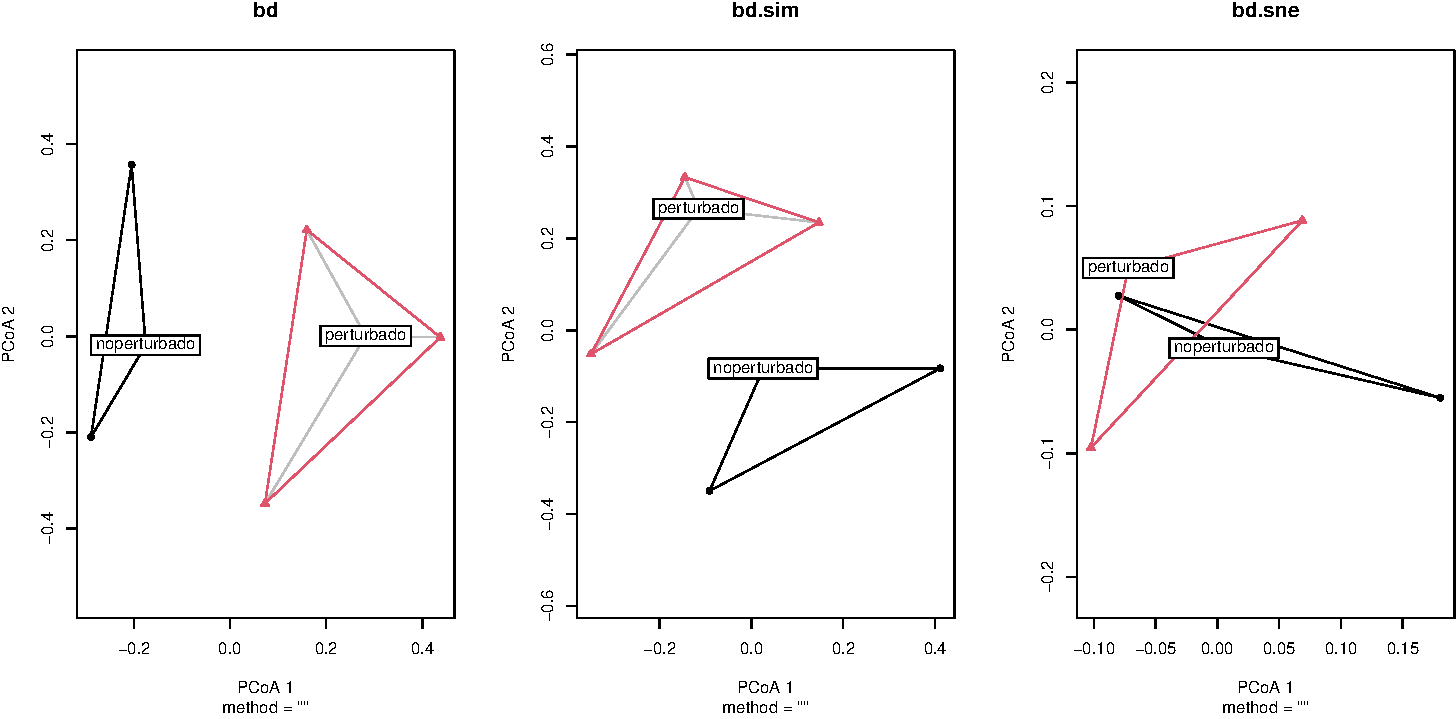
\includegraphics{Clase1-bioest_files/figure-latex/unnamed-chunk-26-1.pdf}

\hfill\break

El gráfico de dispersión beta indica que hay una diferencia en la
composición de especies de los fragmentos de bosque perturbado y no
perturbado. Con estas matrices de distancia luego también podemos
aplicar las diversidad técnicas multivariadas que vimos en el capítulo
pasado como perMANOVA, cluster y los diferentes métodos de ordeniación
para corroborar estas diferencias en composición.

Si queremos obtener estos mismos resultados pero para todos los sitios,
entonces usamos la función \textbf{beta.multi()}:

\begin{Shaded}
\begin{Highlighting}[]
\NormalTok{dist.multi}\OtherTok{\textless{}{-}}\FunctionTok{beta.multi}\NormalTok{(presabs,}\AttributeTok{index.family =}\StringTok{"sorensen"}\NormalTok{ )}
\FunctionTok{head}\NormalTok{(dist.multi)}
\end{Highlighting}
\end{Shaded}

\begin{verbatim}
## $beta.SIM
## [1] 0.4871795
## 
## $beta.SNE
## [1] 0.1206637
## 
## $beta.SOR
## [1] 0.6078431
\end{verbatim}

\hypertarget{ejemplo-aplicado-1}{%
\subsubsection{Ejemplo aplicado}\label{ejemplo-aplicado-1}}

Con la misma data trabajada anteriormente vamos a verificar si dan
resultados similares utilizando el índice de Jaccard.

\newpage

\hypertarget{vegan}{%
\subsection{\texorpdfstring{\texttt{vegan}}{vegan}}\label{vegan}}

Esta paquetería es una excelente herramienta para analizar datos
ecológicos. En el caso de alpha diversidad se pueden calcular los
índices tradicionales (que no están en el marco de los números de Hill).

Aquí realizaremos un ejemplo con una data que trae de ejemplo que se
llama BCI (Barro Colorado Island Tree Counts).

Primero llamamos la data:

\begin{Shaded}
\begin{Highlighting}[]
\FunctionTok{data}\NormalTok{(BCI, BCI.env)}
\end{Highlighting}
\end{Shaded}

Y podemos calcular los índices de diversidad alpha, como Shannon,
Simpson, el inverso de Simpson, Fisher, Especies observadas, beta y
gamma:

\begin{Shaded}
\begin{Highlighting}[]
\NormalTok{shannon }\OtherTok{\textless{}{-}} \FunctionTok{diversity}\NormalTok{(BCI)}
\NormalTok{simpson }\OtherTok{\textless{}{-}} \FunctionTok{diversity}\NormalTok{(BCI, }\StringTok{"simpson"}\NormalTok{)}
\NormalTok{inverso\_simp }\OtherTok{\textless{}{-}} \FunctionTok{diversity}\NormalTok{(BCI, }\StringTok{"inv"}\NormalTok{)}
\NormalTok{fisher }\OtherTok{\textless{}{-}} \FunctionTok{fisher.alpha}\NormalTok{(BCI)}
\NormalTok{especies\_num }\OtherTok{\textless{}{-}} \FunctionTok{specnumber}\NormalTok{(BCI) }

\DocumentationTok{\#\# La diversidad beta definida como gamma/alpha {-} 1:}
\DocumentationTok{\#\# teniendo en cuenta el número total de especies}
\NormalTok{(alpha }\OtherTok{\textless{}{-}} \FunctionTok{with}\NormalTok{(BCI.env, }\FunctionTok{tapply}\NormalTok{(}\FunctionTok{specnumber}\NormalTok{(BCI), Habitat, mean)))}
\end{Highlighting}
\end{Shaded}

\begin{verbatim}
##  OldHigh   OldLow OldSlope    Swamp    Young 
## 85.75000 91.76923 91.58333 94.00000 90.00000
\end{verbatim}

\begin{Shaded}
\begin{Highlighting}[]
\NormalTok{(gamma }\OtherTok{\textless{}{-}} \FunctionTok{with}\NormalTok{(BCI.env, }\FunctionTok{specnumber}\NormalTok{(BCI, Habitat)))}
\end{Highlighting}
\end{Shaded}

\begin{verbatim}
##  OldHigh   OldLow OldSlope    Swamp    Young 
##      158      210      183      128      117
\end{verbatim}

\begin{Shaded}
\begin{Highlighting}[]
\NormalTok{gamma}\SpecialCharTok{/}\NormalTok{alpha }\SpecialCharTok{{-}} \DecValTok{1}
\end{Highlighting}
\end{Shaded}

\begin{verbatim}
##   OldHigh    OldLow  OldSlope     Swamp     Young 
## 0.8425656 1.2883487 0.9981802 0.3617021 0.3000000
\end{verbatim}

\begin{Shaded}
\begin{Highlighting}[]
\DocumentationTok{\#\# de manela similar pero con la diversidad de Shannon}
\NormalTok{(alpha }\OtherTok{\textless{}{-}} \FunctionTok{with}\NormalTok{(BCI.env, }\FunctionTok{tapply}\NormalTok{(}\FunctionTok{diversity}\NormalTok{(BCI), Habitat, mean))) }\CommentTok{\# promedio}
\end{Highlighting}
\end{Shaded}

\begin{verbatim}
##  OldHigh   OldLow OldSlope    Swamp    Young 
## 3.638598 3.876413 3.887122 4.003780 3.246729
\end{verbatim}

\begin{Shaded}
\begin{Highlighting}[]
\NormalTok{(gamma }\OtherTok{\textless{}{-}} \FunctionTok{with}\NormalTok{(BCI.env, }\FunctionTok{diversity}\NormalTok{(BCI, }\AttributeTok{groups=}\NormalTok{Habitat))) }\CommentTok{\# junta}
\end{Highlighting}
\end{Shaded}

\begin{verbatim}
##  OldHigh   OldLow OldSlope    Swamp    Young 
## 3.873186 4.284972 4.212098 4.164335 3.387536
\end{verbatim}

\begin{Shaded}
\begin{Highlighting}[]
\DocumentationTok{\#\# aditiva con la diversidad de Shannon}
\NormalTok{gamma}\SpecialCharTok{{-}}\NormalTok{alpha}
\end{Highlighting}
\end{Shaded}

\begin{verbatim}
##   OldHigh    OldLow  OldSlope     Swamp     Young 
## 0.2345878 0.4085595 0.3249760 0.1605548 0.1408068
\end{verbatim}

Para la beta divesidad podemos calcular nuestras matrices de distancia
con la función `vegdist':

\begin{Shaded}
\begin{Highlighting}[]
\FunctionTok{library}\NormalTok{(tidyverse)}
\NormalTok{distancias}\OtherTok{\textless{}{-}} \FunctionTok{vegdist}\NormalTok{(BCI, }\AttributeTok{method =} \StringTok{"jaccard"}\NormalTok{)}
\NormalTok{distancias }\SpecialCharTok{\%\textgreater{}\%} \FunctionTok{as.matrix}\NormalTok{() }\SpecialCharTok{\%\textgreater{}\%} \FunctionTok{as.data.frame}\NormalTok{() }\SpecialCharTok{\%\textgreater{}\%}\NormalTok{ dplyr}\SpecialCharTok{::}\FunctionTok{select}\NormalTok{(}\DecValTok{1}\SpecialCharTok{:}\DecValTok{4}\NormalTok{) }\SpecialCharTok{\%\textgreater{}\%}\NormalTok{ dplyr}\SpecialCharTok{::}\FunctionTok{slice}\NormalTok{(}\DecValTok{1}\SpecialCharTok{:}\DecValTok{4}\NormalTok{)}
\end{Highlighting}
\end{Shaded}

\begin{verbatim}
##           1         2         3         4
## 1 0.0000000 0.4260250 0.5186992 0.5382263
## 2 0.4260250 0.0000000 0.4463668 0.4790323
## 3 0.5186992 0.4463668 0.0000000 0.4898911
## 4 0.5382263 0.4790323 0.4898911 0.0000000
\end{verbatim}

\hypertarget{parte-2}{%
\section{Parte 2}\label{parte-2}}

\hypertarget{inext}{%
\subsection{iNEXT}\label{inext}}

iNEXT (iNterpolation and EXTrapolation) \footnote{\url{https://github.com/JohnsonHsieh/iNEXT}}

Es un paquete disponible en R para rarefacción y extrapolación de la
diversidad de especies en el marco de los números de Hill. Véase (Chao
and Jost 2012) y (Chao et al. 2014) para metodologías.También está
disponible una versión en línea de iNEXT Online para usuarios sin
experiencia en R.

iNEXT se centra en tres medidas de los números de Hill de orden q:
riqueza de especies (q=0), diversidad de Shannon (q=1, la exponencial de
la entropía de Shannon) y diversidad de Simpson (q=2, la inversa de la
concentración de Simpson).

Para cada medida de diversidad, iNEXT utiliza la muestra observada de
datos de abundancia o incidencia para calcular las estimaciones de
diversidad para muestras enrarecidas y extrapoladas y los intervalos de
confianza del 95 \% (predeterminados) asociados, además de representar
gráficamente los dos tipos siguientes de las curvas de rarefacción y
extrapolación (R/E):

\begin{itemize}
\item
  Curvas de muestreo R/E basadas en el tamaño de la muestra: iNEXT
  calcula estimaciones de diversidad para muestras enrarecidas y
  extrapoladas hasta el doble del tamaño de la muestra de referencia
  (por defecto) o un tamaño especificado por el usuario. Este tipo de
  curva de muestreo traza las estimaciones de diversidad con respecto al
  tamaño de la muestra. El tamaño de la muestra se refiere al número de
  individuos en una muestra para datos de abundancia, mientras que se
  refiere al número de unidades de muestreo para datos de incidencia.
\item
  Curvas de muestreo R/E basadas en la cobertura: iNEXT calcula
  estimaciones de diversidad para muestras enrarecidas y extrapoladas
  con integridad de la muestra (medida por la cobertura de la muestra)
  hasta el valor de cobertura del doble del tamaño de la muestra de
  referencia (por defecto) o una cobertura especificada por el usuario.
  Este tipo de curva de muestreo traza las estimaciones de diversidad
  con respecto a la cobertura de la muestra. Además de los dos tipos
  anteriores de curvas de muestreo, iNEXT también traza una curva de
  completitud de la muestra, que describe cómo varía la estimación de la
  cobertura de la muestra en función del tamaño de la muestra. La curva
  de integridad de la muestra se puede considerar como un puente que
  conecta los dos tipos de curvas mencionados anteriormente.
\end{itemize}

Para instalar este paquete:

\begin{Shaded}
\begin{Highlighting}[]
\DocumentationTok{\#\# instalando iNEXT del CRAN}
\FunctionTok{install.packages}\NormalTok{(}\StringTok{"iNEXT"}\NormalTok{)}

\DocumentationTok{\#\# instalando la versión de desarrollo}
\FunctionTok{install.packages}\NormalTok{(}\StringTok{\textquotesingle{}devtools\textquotesingle{}}\NormalTok{)}
\FunctionTok{library}\NormalTok{(devtools)}
\FunctionTok{install\_github}\NormalTok{(}\StringTok{\textquotesingle{}AnneChao/iNEXT\textquotesingle{}}\NormalTok{)}
\end{Highlighting}
\end{Shaded}

\begin{Shaded}
\begin{Highlighting}[]
\DocumentationTok{\#\# cargando el paquete}
\FunctionTok{library}\NormalTok{(iNEXT)}
\FunctionTok{library}\NormalTok{(ggplot2)}
\end{Highlighting}
\end{Shaded}

\hfill\break

La función principal es:

iNEXT(x, q=0, datatype=``abundance'', se=TRUE, conf=0.95, nboot=50)

Donde:

\begin{itemize}
\item
  x : es la data,
\item
  datatype: puede ser ``abundance'' ó ``incidence\_raw'', ó
  ``incidence\_freq'',
\item
  se: TRUE o FALSE si se quiere hacer un muestreo tipo `bootsrap',
\item
  conf: el intervalo de confianza,
\item
  nboot: número de replicaciones de `bootsrap'
\end{itemize}

Correremos el ejemplo con la data del paquete, denominada
\textbf{spider}:

\begin{Shaded}
\begin{Highlighting}[]
\FunctionTok{data}\NormalTok{(}\StringTok{"spider"}\NormalTok{)}
\FunctionTok{str}\NormalTok{(spider)}
\end{Highlighting}
\end{Shaded}

\begin{verbatim}
## List of 2
##  $ Girdled: num [1:26] 46 22 17 15 15 9 8 6 6 4 ...
##  $ Logged : num [1:37] 88 22 16 15 13 10 8 8 7 7 ...
\end{verbatim}

\begin{Shaded}
\begin{Highlighting}[]
\NormalTok{out }\OtherTok{\textless{}{-}} \FunctionTok{iNEXT}\NormalTok{(spider, }\AttributeTok{q=}\FunctionTok{c}\NormalTok{(}\DecValTok{0}\NormalTok{, }\DecValTok{1}\NormalTok{, }\DecValTok{2}\NormalTok{), }\AttributeTok{datatype=}\StringTok{"abundance"}\NormalTok{)}
\end{Highlighting}
\end{Shaded}

Si vemos el output de iNEXT nos da una lista con tres elementos:

\begin{itemize}
\item
  \$DataInfo que nos resume la información de la data
\item
  \$iNextEst los estimados para las muestras rarificadas y extrapoladas
  (datos para las curvas)
\item
  \$AsyEst muestra la diversidad estimada
\end{itemize}

\begin{Shaded}
\begin{Highlighting}[]
\NormalTok{out}
\end{Highlighting}
\end{Shaded}

\begin{verbatim}
## Compare 2 assemblages with Hill number order q = 0, 1, 2.
## $class: iNEXT
## 
## $DataInfo: basic data information
##      site   n S.obs     SC f1 f2 f3 f4 f5 f6 f7 f8 f9 f10
## 1 Girdled 168    26 0.9289 12  4  0  1  0  2  0  1  1   0
## 2  Logged 252    37 0.9446 14  4  4  3  1  0  3  2  0   1
## 
## $iNextEst: diversity estimates with rarefied and extrapolated samples.
## $Girdled
##       m       method order     qD qD.LCL qD.UCL    SC SC.LCL SC.UCL
## 1     1 interpolated     0  1.000  1.000  1.000 0.122  0.092  0.153
## 10   84 interpolated     0 18.912 15.976 21.848 0.900  0.873  0.926
## 20  168     observed     0 26.000 21.331 30.669 0.929  0.902  0.956
## 30  248 extrapolated     0 30.883 24.501 37.265 0.948  0.917  0.980
## 40  336 extrapolated     0 34.731 26.195 43.267 0.964  0.932  0.995
## 41    1 interpolated     1  1.000  1.000  1.000 0.122  0.092  0.153
## 50   84 interpolated     1 10.964  9.170 12.758 0.900  0.873  0.926
## 60  168     observed     1 12.060  9.947 14.173 0.929  0.899  0.958
## 70  248 extrapolated     1 12.606 10.329 14.884 0.948  0.914  0.982
## 80  336 extrapolated     1 13.014 10.609 15.420 0.964  0.930  0.998
## 81    1 interpolated     2  1.000  1.000  1.000 0.122  0.091  0.154
## 90   84 interpolated     2  7.532  5.841  9.222 0.900  0.868  0.931
## 100 168     observed     2  7.840  5.997  9.683 0.929  0.897  0.960
## 110 248 extrapolated     2  7.945  6.049  9.841 0.948  0.912  0.985
## 120 336 extrapolated     2  8.004  6.077  9.931 0.964  0.927  1.000
## 
## $Logged
##       m       method order     qD qD.LCL qD.UCL    SC SC.LCL SC.UCL
## 1     1 interpolated     0  1.000  1.000  1.000 0.145  0.116  0.173
## 10  126 interpolated     0 28.268 25.439 31.097 0.908  0.888  0.928
## 20  252     observed     0 37.000 32.195 41.805 0.945  0.922  0.967
## 30  371 extrapolated     0 42.786 35.837 49.734 0.958  0.933  0.982
## 40  504 extrapolated     0 47.644 38.051 57.238 0.969  0.945  0.993
## 41    1 interpolated     1  1.000  1.000  1.000 0.145  0.108  0.181
## 50  126 interpolated     1 13.172 10.837 15.507 0.908  0.887  0.930
## 60  252     observed     1 14.421 11.762 17.080 0.945  0.924  0.966
## 70  371 extrapolated     1 15.010 12.201 17.820 0.958  0.933  0.983
## 80  504 extrapolated     1 15.457 12.534 18.381 0.969  0.944  0.994
## 81    1 interpolated     2  1.000  1.000  1.000 0.145  0.101  0.188
## 90  126 interpolated     2  6.610  4.777  8.443 0.908  0.886  0.930
## 100 252     observed     2  6.761  4.834  8.689 0.945  0.921  0.968
## 110 371 extrapolated     2  6.812  4.852  8.771 0.958  0.931  0.985
## 120 504 extrapolated     2  6.840  4.863  8.817 0.969  0.942  0.996
## 
## 
## $AsyEst: asymptotic diversity estimates along with related statistics.
##      Site         Diversity Observed Estimator   s.e.    LCL     UCL
## 1 Girdled  Species richness   26.000    43.893 14.306 30.511  96.971
## 2 Girdled Shannon diversity   12.060    13.826  1.467 12.060  16.702
## 3 Girdled Simpson diversity    7.840     8.175  0.983  7.840  10.102
## 4  Logged  Species richness   37.000    61.403 18.532 43.502 128.583
## 5  Logged Shannon diversity   14.421    16.337  1.523 14.421  19.322
## 6  Logged Simpson diversity    6.761     6.920  0.921  6.761   8.726
## 
## NOTE: Only show five estimates, call iNEXT.object$iNextEst. to show complete output.
\end{verbatim}

\begin{itemize}
\tightlist
\item
  Podemos obtener ahora nuestras curvas por sitio o en este caso por
  tratamiento a los 3 órdenes:
\end{itemize}

\begin{Shaded}
\begin{Highlighting}[]
\FunctionTok{ggiNEXT}\NormalTok{(out, }\AttributeTok{type=}\DecValTok{1}\NormalTok{, }\AttributeTok{facet.var=}\StringTok{"site"}\NormalTok{)}
\end{Highlighting}
\end{Shaded}

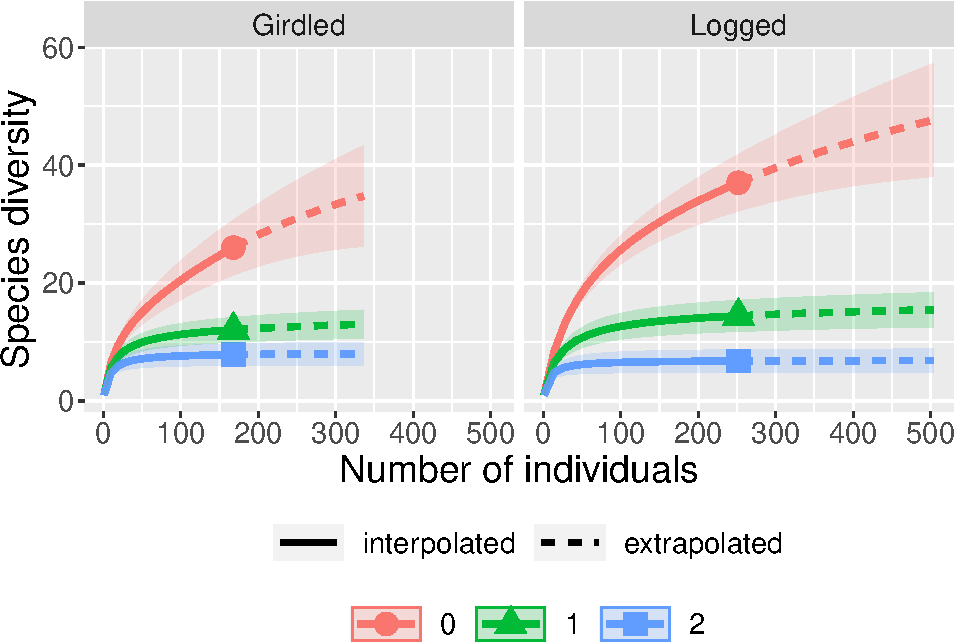
\includegraphics{Clase1-bioest_files/figure-latex/unnamed-chunk-35-1.pdf}

\newpage

\begin{itemize}
\tightlist
\item
  También podemos obtener ahora nuestras curvas de cobertura:
\end{itemize}

\begin{Shaded}
\begin{Highlighting}[]
\FunctionTok{ggiNEXT}\NormalTok{(out, }\AttributeTok{type=}\DecValTok{2}\NormalTok{)}
\end{Highlighting}
\end{Shaded}

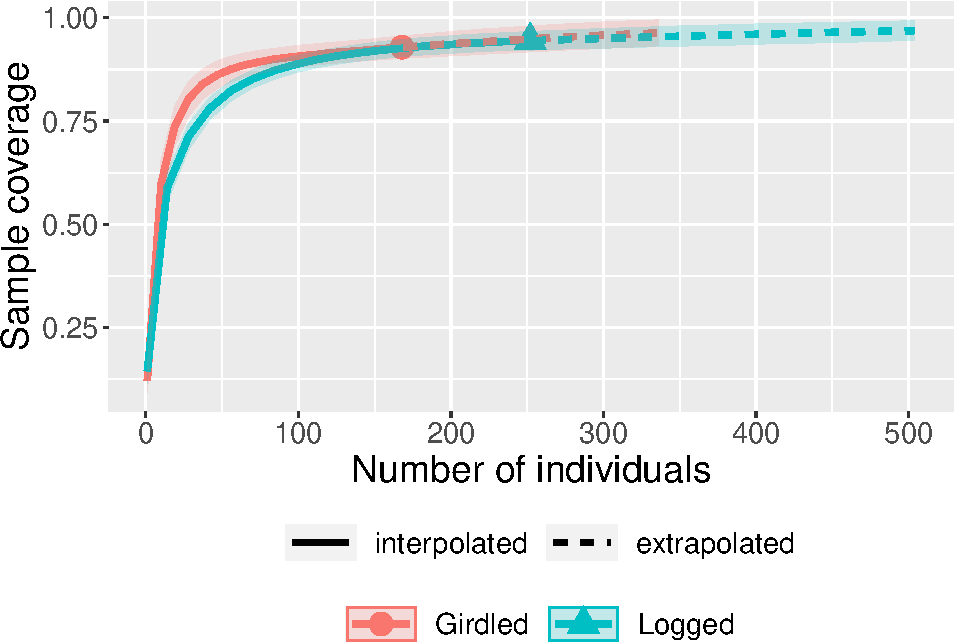
\includegraphics{Clase1-bioest_files/figure-latex/unnamed-chunk-36-1.pdf}

\newpage

\begin{itemize}
\tightlist
\item
  Por último una gráfica de diversidad de especies vs cobertura para los
  tratamientos:
\end{itemize}

\begin{Shaded}
\begin{Highlighting}[]
\FunctionTok{ggiNEXT}\NormalTok{(out, }\AttributeTok{type=}\DecValTok{3}\NormalTok{, }\AttributeTok{facet.var=}\StringTok{"site"}\NormalTok{)}
\end{Highlighting}
\end{Shaded}

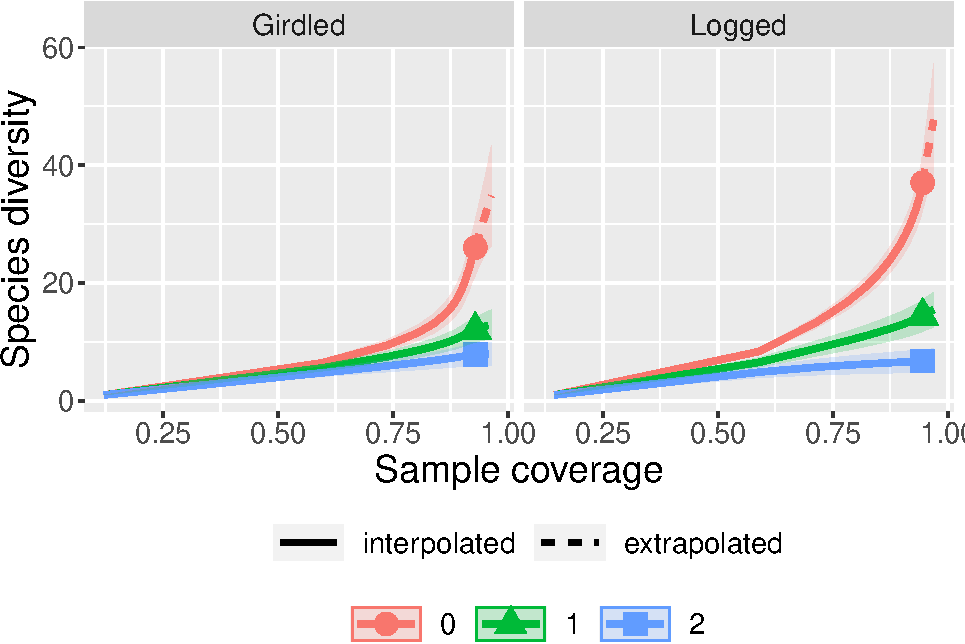
\includegraphics{Clase1-bioest_files/figure-latex/unnamed-chunk-37-1.pdf}

\newpage

\begin{itemize}
\tightlist
\item
  Y a los diferentes órdenes:
\end{itemize}

\begin{Shaded}
\begin{Highlighting}[]
\FunctionTok{ggiNEXT}\NormalTok{(out, }\AttributeTok{type=}\DecValTok{3}\NormalTok{, }\AttributeTok{facet.var=}\StringTok{"order"}\NormalTok{)}
\end{Highlighting}
\end{Shaded}

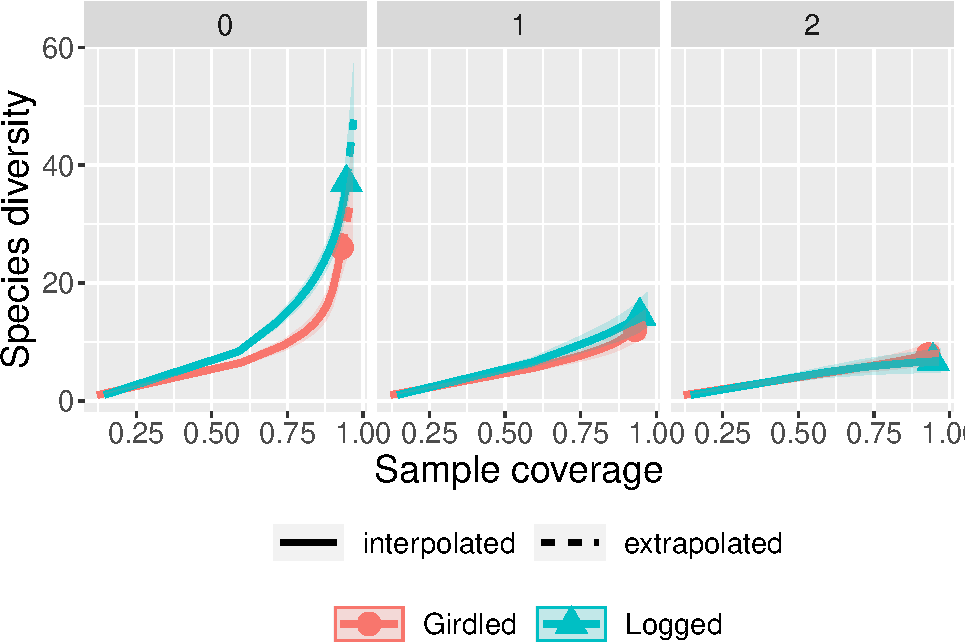
\includegraphics{Clase1-bioest_files/figure-latex/unnamed-chunk-38-1.pdf}

\newpage

Ahora si se quiere sólo los índices basandonos ya sea en abundancia o
incidencia y en tamaño o cobertura, usamos la función
\textbf{estimateD}, así:

\begin{Shaded}
\begin{Highlighting}[]
\FunctionTok{estimateD}\NormalTok{(spider}\SpecialCharTok{$}\NormalTok{Logged, }\AttributeTok{datatype=}\StringTok{"abundance"}\NormalTok{, }\AttributeTok{base=}\StringTok{"size"}\NormalTok{,  }\AttributeTok{conf=}\FloatTok{0.95}\NormalTok{)}
\end{Highlighting}
\end{Shaded}

\begin{verbatim}
##     m   method order    SC     qD qD.LCL qD.UCL
## 1 252 observed     0 0.945 37.000 31.322 42.678
## 2 252 observed     1 0.945 14.421 11.757 17.085
## 3 252 observed     2 0.945  6.761  5.041  8.482
\end{verbatim}

\begin{Shaded}
\begin{Highlighting}[]
\FunctionTok{estimateD}\NormalTok{(spider}\SpecialCharTok{$}\NormalTok{Girdled, }\AttributeTok{datatype=}\StringTok{"abundance"}\NormalTok{, }\AttributeTok{base=}\StringTok{"size"}\NormalTok{,  }\AttributeTok{conf=}\FloatTok{0.95}\NormalTok{)}
\end{Highlighting}
\end{Shaded}

\begin{verbatim}
##     m   method order    SC    qD qD.LCL qD.UCL
## 1 168 observed     0 0.929 26.00 20.338 31.662
## 2 168 observed     1 0.929 12.06  9.927 14.192
## 3 168 observed     2 0.929  7.84  6.110  9.570
\end{verbatim}

\hfill\break

\hypertarget{ejemplo-aplicado-2}{%
\subsubsection{Ejemplo aplicado}\label{ejemplo-aplicado-2}}

Apliquemos lo visto usando como ejemplo pequeño con datos de incidencia
(presencia/ausencia):

\begin{Shaded}
\begin{Highlighting}[]
\FunctionTok{data}\NormalTok{(ciliates)}
\CommentTok{\#str(ciliates)}
\end{Highlighting}
\end{Shaded}

\hfill\break

Este paquete también cuenta con otras funciones de interés, tales como:

\begin{itemize}
\item
  ChaoEntropy() : Estimación de la entropía/diversidad de Shannon
\item
  ChaoRichness(): Estimación de la riqueza de especies
\item
  ChaoShannon(): Estimación de la entropía/diversidad de Shannon
\item
  ChaoSimpson(): Estimación del índice de Gini-Simpson o diversidad de
  Simpson
\item
  ChaoSpecies(): Estimación de la riqueza de especies
\item
  EstSimpson: Estimación del índice de Gini-Simpson o diversidad de
  Simpson
\end{itemize}

\hfill\break

Un ejemplo:

\begin{Shaded}
\begin{Highlighting}[]
\FunctionTok{ChaoRichness}\NormalTok{(spider)}
\end{Highlighting}
\end{Shaded}

\begin{verbatim}
##         Observed Estimator Est_s.e. 95% Lower 95% Upper
## Girdled       26    43.893   14.306    30.511    96.971
## Logged        37    61.403   18.532    43.502   128.583
\end{verbatim}

\begin{Shaded}
\begin{Highlighting}[]
\FunctionTok{ChaoShannon}\NormalTok{(spider)}
\end{Highlighting}
\end{Shaded}

\begin{verbatim}
##         Observed Estimator Est_s.e 95% Lower 95% Upper
## Girdled    2.490     2.627   0.110     2.490     2.842
## Logged     2.669     2.793   0.099     2.669     2.988
\end{verbatim}

\hypertarget{curvas-en-vegan}{%
\subsection{Curvas en vegan}\label{curvas-en-vegan}}

\begin{Shaded}
\begin{Highlighting}[]
\FunctionTok{library}\NormalTok{(vegan)}
\FunctionTok{data}\NormalTok{(}\StringTok{"BCI"}\NormalTok{)}
\FunctionTok{head}\NormalTok{(BCI)[}\DecValTok{1}\SpecialCharTok{:}\DecValTok{4}\NormalTok{,}\DecValTok{1}\SpecialCharTok{:}\DecValTok{4}\NormalTok{]}
\end{Highlighting}
\end{Shaded}

\begin{verbatim}
##   Abarema.macradenia Vachellia.melanoceras Acalypha.diversifolia
## 1                  0                     0                     0
## 2                  0                     0                     0
## 3                  0                     0                     0
## 4                  0                     0                     0
##   Acalypha.macrostachya
## 1                     0
## 2                     0
## 3                     0
## 4                     0
\end{verbatim}

\begin{Shaded}
\begin{Highlighting}[]
\CommentTok{\#por sitios}
\NormalTok{sac }\OtherTok{\textless{}{-}} \FunctionTok{specaccum}\NormalTok{(BCI)}
\FunctionTok{plot}\NormalTok{(sac, }\AttributeTok{ci.type=}\StringTok{"polygon"}\NormalTok{) }\CommentTok{\#ver vegan para opciones}
\end{Highlighting}
\end{Shaded}

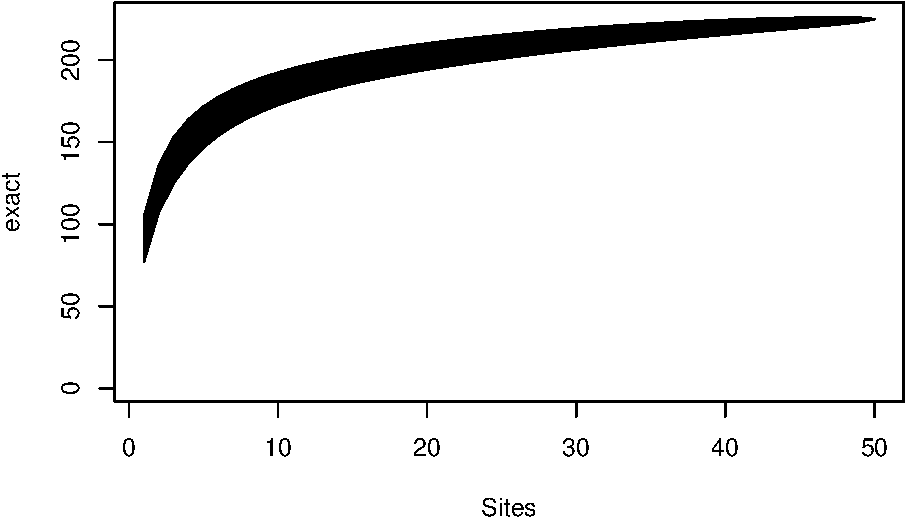
\includegraphics{Clase1-bioest_files/figure-latex/unnamed-chunk-44-1.pdf}

\begin{Shaded}
\begin{Highlighting}[]
\CommentTok{\#por individuos}
\NormalTok{sac }\OtherTok{\textless{}{-}} \FunctionTok{specaccum}\NormalTok{(BCI, }\AttributeTok{method =} \StringTok{"rarefaction"}\NormalTok{)}
\FunctionTok{plot}\NormalTok{(sac, }\AttributeTok{xvar =} \StringTok{"individual"}\NormalTok{, }\AttributeTok{ci.type=}\StringTok{"polygon"}\NormalTok{) }
\end{Highlighting}
\end{Shaded}

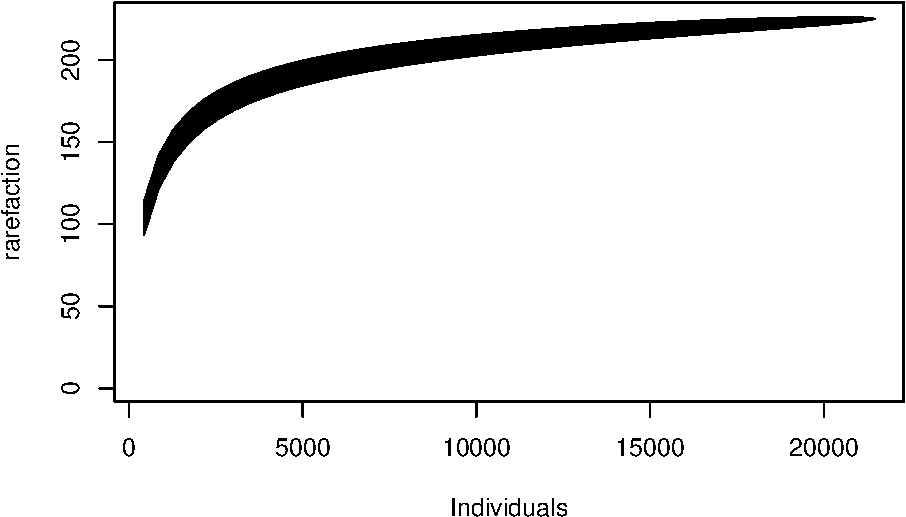
\includegraphics{Clase1-bioest_files/figure-latex/unnamed-chunk-44-2.pdf}

\newpage

\hypertarget{referencias}{%
\section{REFERENCIAS}\label{referencias}}

\hfill\break

\hypertarget{refs}{}
\begin{CSLReferences}{1}{0}
\leavevmode\vadjust pre{\hypertarget{ref-baselga2012}{}}%
Baselga, Andrés, and C. David L. Orme. 2012. {``Betapart : An R Package
for the Study of Beta Diversity.''} \emph{Methods in Ecology and
Evolution} 3 (5): 808--12.
\url{https://doi.org/10.1111/j.2041-210x.2012.00224.x}.

\leavevmode\vadjust pre{\hypertarget{ref-chao2014a}{}}%
Chao, Anne, Chun-Huo Chiu, and Lou Jost. 2014. {``Unifying Species
Diversity, Phylogenetic Diversity, Functional Diversity, and Related
Similarity and Differentiation Measures Through Hill Numbers.''}
\emph{Annual Review of Ecology, Evolution, and Systematics} 45 (1):
297--324. \url{https://doi.org/10.1146/annurev-ecolsys-120213-091540}.

\leavevmode\vadjust pre{\hypertarget{ref-chao2014}{}}%
Chao, Anne, Nicholas J. Gotelli, T. C. Hsieh, Elizabeth L. Sander, K. H.
Ma, Robert K. Colwell, and Aaron M. Ellison. 2014. {``Rarefaction and
Extrapolation with Hill Numbers: A Framework for Sampling and Estimation
in Species Diversity Studies.''} \emph{Ecological Monographs} 84 (1):
45--67. \url{https://doi.org/10.1890/13-0133.1}.

\leavevmode\vadjust pre{\hypertarget{ref-Chao2012}{}}%
Chao, Anne, and Lou Jost. 2012. {``Coverage-Based Rarefaction and
Extrapolation: Standardizing Samples by Completeness Rather Than
Size.''} \emph{Ecology} 93 (12): 2533--47.
\url{https://doi.org/10.1890/11-1952.1}.

\leavevmode\vadjust pre{\hypertarget{ref-Chiu2014}{}}%
Chiu, Chun-Huo, and Anne Chao. 2014. {``Distance-Based Functional
Diversity Measures and Their Decomposition: A Framework Based on Hill
Numbers.''} Edited by Francesco de Bello. \emph{PLoS ONE} 9 (7):
e100014. \url{https://doi.org/10.1371/journal.pone.0100014}.

\leavevmode\vadjust pre{\hypertarget{ref-sackett2011}{}}%
Sackett, Tara E., Sydne Record, Sharon Bewick, Benjamin Baiser, Nathan
J. Sanders, and Aaron M. Ellison. 2011. {``Response of Macroarthropod
Assemblages to the Loss of Hemlock ({\emph{Tsuga Canadensis}}), a
Foundation Species.''} \emph{Ecosphere} 2 (7): art74.
\url{https://doi.org/10.1890/es11-00155.1}.

\end{CSLReferences}

\end{document}
